\documentclass{beamer}

\usepackage{minted}
\usepackage{pgf}
\usepackage[utf8]{inputenc}
\usepackage{mdframed}

\BeforeBeginEnvironment{minted}{\begin{mdframed}}
\AfterEndEnvironment{minted}{\end{mdframed}}

\title{Let The Compiler Help You: How To Make The Most Of Scala's Typesystem}
\author{Markus Hauck (@markus1189)}

\date{Scala.IO 2017}
\subject{Computer Science}
\usetheme{codecentric}

\renewcommand\texttt[1]{\mintinline{scala}/#1/}

\usemintedstyle{fruity}

\begin{document}

{
  \usebackgroundtemplate{
\includegraphics[height=\paperheight]{background.jpg}}
  \frame[plain]{\titlepage}
}

\section{Intro}
\label{sec:intro}

\begin{frame}
  \frametitle{Introduction}
  \begin{itemize}
  \item Programming as a dialog between you and the compiler
  \item Compiler tells you that what you wrote makes sense
  \item Tries to prevent you from making errors
  \item Ultimately you run and see whether it works
  \item Hate/love relationship with the compiler
  \end{itemize}
\end{frame}

\begin{frame}
  \frametitle{Become Friends}
  \begin{itemize}
  \item Turns out the compiler is only there to help
  \item He wants you to succeed, not prevent you to
  \item You should write your code in a way that the compiler can do
    the most for you
  \item This talk: how to improve your relationship with your compiler
  \end{itemize}
\end{frame}

\begin{frame}
  \frametitle{Disclaimer: The Compiler. Does. Not. Read. Documentation}
  \begin{itemize}
  \item documentation is NOT a way to talk to your compiler
  \item (and probably neither to your coworkers)
  \item also to avoid: \textbf{context sensitive} reasoning
  \item think: I \textbf{know} this can't happen
  \item use a language that the compiler understands: types
  \end{itemize}
\end{frame}

\section{Step 1: Don't lie}

\begin{frame}[c]
  \begin{center}
    \Large Step 1: Don't lie about what you CAN do
  \end{center}
\end{frame}

\begin{frame}[fragile]
  \frametitle{Get The Max Out Of Your List}
  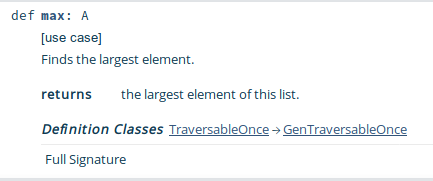
\includegraphics[width=0.8\textwidth]{../pics/list-max.png}
\end{frame}

\begin{frame}[fragile,fragile]
  \frametitle{Putting It Into Practice}
  \begin{minted}{scala}
> List[Int](1, 2, 3).max
res0: Int = 3
\end{minted}
\begin{minted}{scala}
> List[Int]().max                                                             
java.lang.UnsupportedOperationException: empty.max                                 
\end{minted}
\end{frame}

\begin{frame}
  \frametitle{Step 1: Don't lie about what you can do}
  \begin{itemize}
  \item The compiler can't help you if you lie
  \item How to tell the truth:
    \begin{itemize}
    \item Option
    \item Either
    \item Custom ADT
    \end{itemize}
  \end{itemize}
\end{frame}

\begin{frame}
  \frametitle{A better max}
  
\end{frame}

\section{Step 2: If not allowed, forbid it}

\begin{frame}[fragile]
  \frametitle{If not allowed, FORBID it}
\begin{minted}{scala}
case class Email(value: String) extends AnyVal {
  require(isValidEmail(value))
}
\end{minted}
\begin{minted}{scala}
> Email("markus.hauck@codecentric.de")
res1: Email = ...
> Email("Hello World!")
java.lang.IllegalArgumentException: 
  Not a valid email address                      
\end{minted}
\end{frame}

\begin{frame}[fragile,fragile]
  \frametitle{If not allowed, FORBID it}
\begin{minted}{scala}
abstract case class Email private (...)

object Email {
  def fromString: Either[ValidationError, Email] = 
    ??? // exercise
}
\end{minted}

\begin{minted}{scala}
> Email.fromString("markus.hauck@codecentric.de")
res1: Either[ValidationError, Email] = 
  Right("markus.hauck@codecentric.de")

> Email.fromString("Hello World")
res2: Either[ValidationError, Email] = 
  Left(InvalidEmail)
\end{minted}
\end{frame}

\begin{frame}
  \frametitle{Ensure Simple Invariants}
  \begin{itemize}
  \item let's start with ensuring invariants
  \item two ways to react to invalid input:
    \begin{itemize}
    \item signal error (as return value)
    \item better: don't allow invalid input!
    \end{itemize}
  \end{itemize}
\end{frame}

\section{Step 3: Don't accept garbage}

\begin{frame}
  \frametitle{Step 3: Don't accept garbage}
  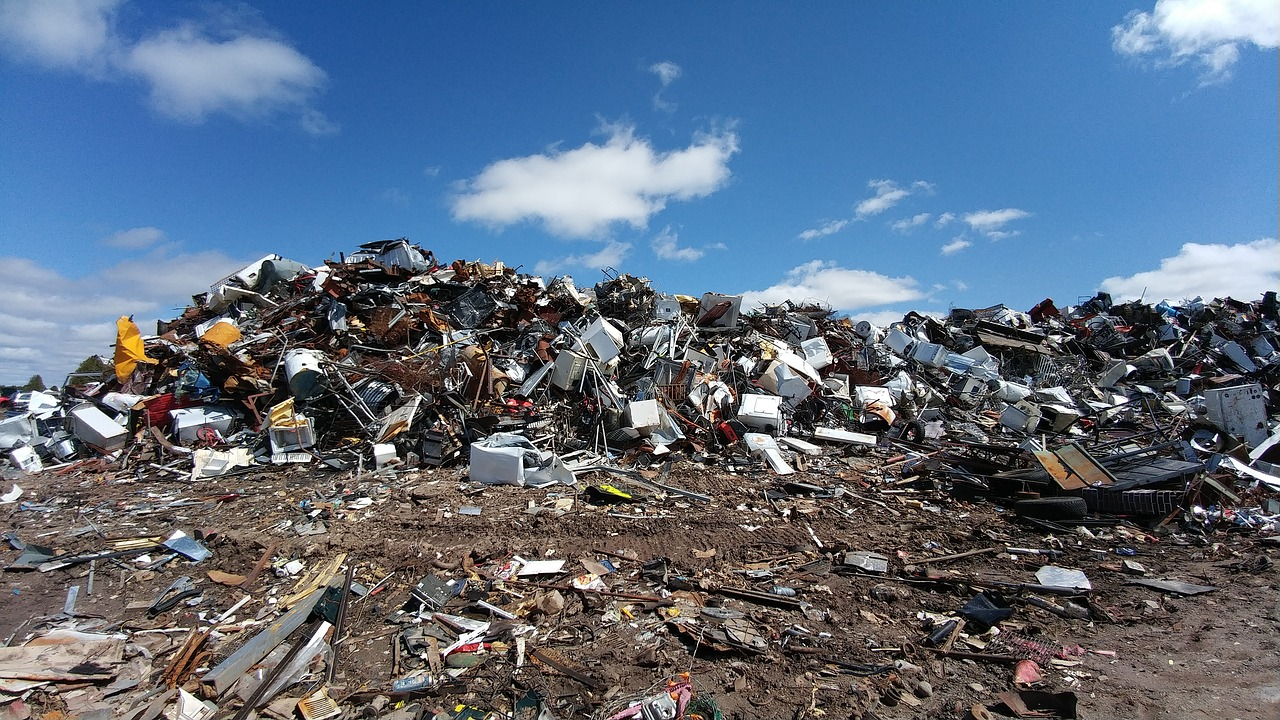
\includegraphics[width=\textwidth]{../pics/scrapyard-2441432_1280.jpg}
\end{frame}

\begin{frame}
  \frametitle{Avoid Invalid Instantiation}
  \begin{itemize}
  \item require/assert/exceptions = bad
  \item better: use custom instantiation methods
  \end{itemize}
\end{frame}

\begin{frame}
  \frametitle{Don't accept garbage as your input}
   \begin{itemize}
  \item previously: accept arguments, maybe fail
  \item but: we did nothing wrong!  It's the caller's fault!
  \item use types to only accept valid input
  \item (this is a trade-off and cannot be done for all args)
  \item negative int, empty collection and more
  \item how to enforce?
    \begin{itemize}
    \item custom classes with smart constructors
    \item if possible use libraries
    \end{itemize}
  \end{itemize}
\end{frame}

\begin{frame}
  \frametitle{Pushing Boundaries}
  \begin{itemize}
  \item we shift the responsiblity to another place
  \item good: separate \textit{validation} from actual program
  \item goal: push it to the boundaries and deal with it \textbf{once}
  \end{itemize}
\end{frame}

\begin{frame}[fragile,fragile]
  \frametitle{Putting It Into Practice}
\begin{minted}{scala}
def sendEmail(mail: String): Either[MailValidationError, MailStatus]
// vs
def sendEmail(mail: Email): MailStatus
\end{minted}
\begin{minted}{scala}
> NonEmptyList.of(1, 2, 3).head
res1: Int = 1
\end{minted}
\end{frame}

\section{Step 4: Avoid Inconsistent States}

\begin{frame}
  \frametitle{Phantom Types for Tags}
  \begin{itemize}
  \item Creating new classes for invariants works, but very cumbersome
  \item But: Whenever input enters your system: require validation
  \item Avoid validation again and again because of different flows
    through system and refactorings (context-free!)
  \end{itemize}
\end{frame}

\begin{frame}
  \frametitle{Refined}
  \begin{itemize}
  \item Indexing into collections
  \item Creating e.g. Versions from Strings
  \item Calculate average on empty list?
  \item Validation should happen \textbf{at the boundaries} (once and
    for all)
  \end{itemize}
\end{frame}

\begin{frame}
  \frametitle{Phantom Types for State Machines}
  \begin{itemize}
  \item Given a state machine type of flow, we can represent that with
    types!
  \item Use subtyping to model your graph
  \item typical example: the builder
  \end{itemize}
\end{frame}

\begin{frame}
  \frametitle{Calculate Types}
  
\end{frame}

\begin{frame}
  \frametitle{The Compiler Is There To Help!}
  \vfill
  \begin{center}
    {\Huge THANKS!}
  \end{center}
\end{frame}

\end{document}
